%
% File naaclhlt2016.tex
%

\documentclass[11pt,letterpaper]{article}
\usepackage{naaclhlt2016}
\usepackage{times}
\usepackage{graphicx}
\usepackage{subcaption}
\captionsetup{compatibility=false}
\graphicspath{ {images/} }

\usepackage{latexsym}
% \naaclfinalcopy % Uncomment this line for the final submission
\def\naaclpaperid{***} %  Enter the naacl Paper ID here

% To expand the titlebox for more authors, uncomment
% below and set accordingly.
% \addtolength\titlebox{.5in}    

\newcommand\BibTeX{B{\sc ib}\TeX}


\title{Program Generation from Natural Languages}

% Author information can be set in various styles:
% For several authors from the same institution:
% \author{Author 1 \and ... \and Author n \\
%         Address line \\ ... \\ Address line}
% if the names do not fit well on one line use
%         Author 1 \\ {\bf Author 2} \\ ... \\ {\bf Author n} \\
% For authors from different institutions:
% \author{Author 1 \\ Address line \\  ... \\ Address line
%         \And  ... \And
%         Author n \\ Address line \\ ... \\ Address line}
% To start a seperate ``row'' of authors use \AND, as in
% \author{Author 1 \\ Address line \\  ... \\ Address line
%         \AND
%         Author 2 \\ Address line \\ ... \\ Address line \And
%         Author 3 \\ Address line \\ ... \\ Address line}
% If the title and author information does not fit in the area allocated,
% place \setlength\titlebox{<new height>} right after
% at the top, where <new height> can be something larger than 2.25in
% \author{Margaret Mitchell \and Adam Lopez\\
  % {\tt naacl-pub-chairs@googlegroups.com}}

% https://github.com/acl-org/acl-pub/blob/gh-pages/paper_styles/archive/naaclhlt2016-latex/naaclhlt2016.pdf
\author{Allan Wang \and Youngsun Jin \\
        McGill University \\ \tt{\{allan.wang,youngsun.jin\}@mail.mcgill.ca}}  
\date{}

\begin{document}

\maketitle

\begin{abstract}
  When learning new programming languages, it is often easy to understand the syntax and learn
  about idiomatic executions through examples. Particularly with different paradigms, how we
  write code in one language may not be one to one with code in another language. Most
  languages provide examples through a list of common executions. If we can instead provide an
  example matching simple instructions in English, we can help refine the amount of code
  a new developer has to go through, and assist in creating an infinite set of examples tailored to
  each user. In this work, we have developed a prototype system which is able to process natural language instructions
  related to list creation with optional conditions, which is then translated into executable code with programming language provided by the user.
\end{abstract}

\section{Introduction}
Learning the syntax of a programming language can be frustrating and challenging. 
For a new developer, programming languages contain lots of domain-specific rules, varying in control structures, syntax, etc.
For experienced developers, programming languages may introduce completely new paradigms, and may not be easily translated from known languages through one to one mappings of keywords.
One way to help overcome this technical hurdle is to read official documentation, or a large set of common examples.
However, this is often a big time investment for a user who just wants to explore the basics of a language.
Moreover, the examples may not completely reflect the desired use case, and can often be irrelevant to the problem at hand.\\

Our goal is to explore the feasibility of mapping natural languages to programs by extracting features and creating runnable code.
This would greatly reduce the learning curve when dealing with simple operations, and will help introduce language features without the developer knowing about them beforehand.
More specifically, we wish to focus on generating number lists in multiple programming languages, allowing for varying constraints available across all supported languages.
We will use Combinatory Categorial Grammar (CCG) to create a tree representing the logic, then introduce language specific transformers to map subtrees to working code.
Lastly, we will pass through the generated body and output a working program.
On top of being able to create a program, we wish to introduce a structure that can be extended to support both new languages and new operations within the semantics tree.

% TODO should we give an example?
% Main goal of intro is to have the hypothesis, which is above   

\section{Related Work}

\subsection{Natural Language to Database Query}

One of the earliest system that makes use of natural language translation into executable code is a Natural Language Interface
for a Database (NLIDB) (Androutsopouloset al., 1995). When databases contain an enormous number records, a specific query language such as the Structured Query Language (SQL) needs to be used in order to extract specific records specified by the expert user. This means that one needs to understand the syntax for querying the database and the way to join the underlying tables to extract necessary records. However, this introduces difficulties for users because they may not be aware of the structure of the database. A NLIDB simplifies the task by providing the user interface to input natural languages to query the database. We can clearly see how this is similar to our task. We want to take natural language as an input, and output equivalent executable code in the user-specified language which returns a collection of entities with some conditions specified by the user. For feasibility, we have simplified the problem to creating a list of numbers with conditions that can be applied to each number inside the list.   

\subsection{Natural Language to Java}
NaturalJava (Price et al., 2000) is one of the early systems that 
allows to create Java programs from English commands. The system accepts English sentences as input and then uses information extraction techniques to map one of 400 case frames. Then the interpreter infers changes that have to be made using a decision tree, which then manipulates Java abstract syntax tree (AST). The AST is automatically converted into Java source code. Although our task is similar in a sense that both translate natural language into code, we do not manually create case frames to infer programs. Our task is more involved with parsing the natural language sentence using a set of rules to generate semantic representation of the input.

\subsection{Unrestricted Natural Language}
One of the most powerful natural language interface was developed (David et al., 2006). They presented the prototype system which takes unrestricted English as input and output code in the Python programming language. They used Combinatory Categorial Grammar (CCG) as a base tool to generate syntactic categories for English sentences. Then the \textit{ccg2sem} system (Bos et al., 2004; Black-burn and Bos, 2005) was used to convert CCG parse trees into Discourse Representation Structure (DRS). Having extracted the functional verb and its arguments, if the semantic information matches with predefined primitives, then the equivalent code is generated. Unlike our task, they trained the new model for the parser on the manually-generated corpus as a result of the differences between standard English sentences and programming statements. However, in this work, we predefined the set of rules in CCG to assign each word with functional feature instead of syntactic category, which will be then used to generate the semantic representation of the whole sentence.

\section{Methodology}

\begin{figure*}[t]
  \small
  \begin{verbatim}
            list                  from         0         to          100
((L/RF)/RT) {\y x.list(x,y)}  (RF/I) {\x.x}  I {0}  (RT/I) {\x.x}  I {100}
                              ---------------------->
                                      RF {0}
                              ----------------------<T
                              (L\(L/RF)) {\F.F(0)}
----------------------------------------------------<B
              (L/RT) {\y.list(0,y)}
                                                    ------------------------>
                                                            RT {100}
---------------------------------------------------------------------------->
                              L {list(0,100)}
  \end{verbatim}
  \caption{\label{font-figure} Shortened example of CCG output.}
\end{figure*}

\subsection{CCG Parsing}

In creating our grammar, we defined a set of rules for each type we may encounter. 
We have the following primitives: {\small\verb|program|}, {\small\verb|creation|}, and {\small\verb|range|}.
A program represents an independent set of rules that is capable or defining a runnable program.
A creation denotes a rule that generates new data. 
This can be any viable programming type, but in our case specifically, it represents an integer list.
A range represents a phrase with a minimum number and maximum number.
This is necessary in creating a proper list.\\

For conditions, we can create higher order types that build upon existing lists.
For instance, an `even list from 0 to 100' would still represent ths {\small\verb|list|} primitive, with a new feature attached.
Here, we begin to face some problems.
We can for instance want a `list from 0 to 100 that is divisible by 4', but a `divisible by 4 list from 0 to 100' would not make sense.
We can work around this by introducing special groups per condition, and making sure that our program rules respect the expected groups based on the order of the initial sentence.\\

Another problem we face is supporting number parsing, where a number primitive can be any valid sequence of digits. 
One way we considered was post processing, where we would replace each number with a special symbol, create our tree, then add back the numbers in the same order as they appeared in the sentence.
This poses a problem, as our assumption of word order may not always be correct. As an example, both `create a list from 0 to 100' and `create a list to 100 from 0' are represented by the same tree, and yet the numbers are not in the same order.
We worked around this by extracting all the numbers in the word token, adding rules that map them to the same integer primitive, and then creating a new ccg parser for each sentence.\\

The final result allows us to create CCGs like in figure 1.
\subsection{Language Formatting}

As we wish to parse our input using a CCG, we must first ensure that our corpus is contained in our lexicon.
We can simply do so be removing all words that are not part of our lexicon, but that would greatly constrain our input, and may also result in code that does not represent what we wanted.
To support a wider set of tokens, we will preprocess the text with a dictionary of token words to NLTK lemma keys.
We can use the keys to extract synonyms, and provided that each word is unique to a specific token, we can replace them without altering the semantics.

We still need to filter out the remaining words, but in checking the part of speeches, we noted that condition features typically contain an adjective or adverb.
We can therefore filter out words without those part of speeches, and return an error when other unknown tokens are found.
This allows us to parse instructions beyond the keywords that we select, and allows us to reject inputs that we cannot parse with reasonable confidence.

\subsection{Feature Mapping}

Once we have our semantics tree, we can map them into programming rules.
By the way we defined our primitives, it is noted that each node can lead to a part of a programming with the information within its subtree.
As we are familiar with both the number of children per primitive, as well as their orders, we can create code templates that take in child subcomponents and generate a new subcomponent.
Once we get to the program primitive, the result should be a working program.

\subsection{Code Generation}

Given that our feature mapping aims to convert a semantics tree to code, our code generation is essentially applying our feature map to the root node.
However, the process is not so simple.
A common part of many programming languages is a set of import rules at the top of the file.
While we can add each rule in our template if they don't appear elsewhere in the subtree, this can quickly become messy for large trees.
A simpler method is to aggregate all necessary imports, and to post process our code to ensure we add unique imports.
We did so by introducing a variable in our feature map output, so that each token is mapped to both a template and an import set.\\

It is worth noting that method is quite extensible, as it does not affect the generation of our program body.
We can almost view it as a new feature tree, where we can define a new mapping to further convert it into code.
In the case of imports, the mapping per node is to simply aggregate the unique key set and to output each of them in a new line.

\begin{figure*}[t!]
    \centering
    \begin{subfigure}[t]{0.5\textwidth}
        \centering
        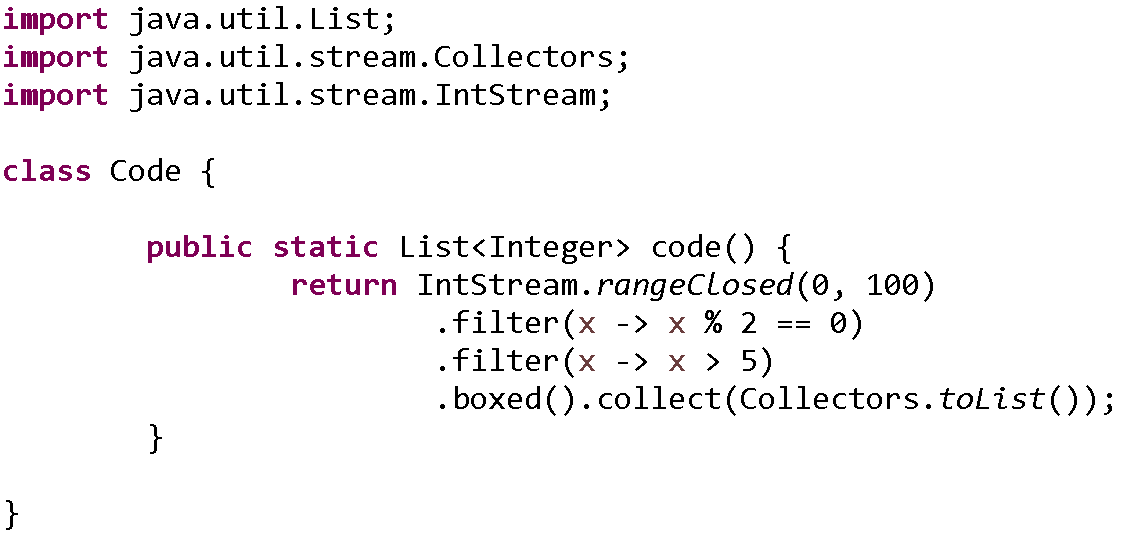
\includegraphics[height=1.2in]{java}
        \caption{Java}
    \end{subfigure}%
    ~ 
    \begin{subfigure}[t]{0.5\textwidth}
        \centering
        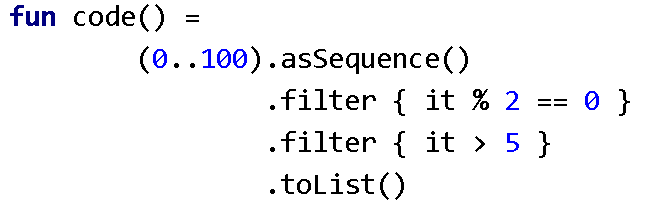
\includegraphics[height=0.8in]{kotlin}
        \caption{Kotlin}
    \end{subfigure}
    
    \caption{Output of \lq create even list from 0 to 100 that is bigger than 5'}
\end{figure*}

\subsection{Negation Extension}

To test the extensibility of our implementation, we implemented negation using our existing structure.
We may note that a negation can take place before any existing condition, and will result in a new predicate with the opposite output.
Furthermore, as an optimization, two consecutive negations will cancel out. 
While we could preprocess the text and remove consecutive negations, we decided to handle this within the parse tree.
To support the negation feature, we will add another attribute in our feature map for conditions only.
When we encounter a negation feature in our tree, we will simply take the child and flip the negation field.
Note that this does mean that we have to apply our template function lazily, as we can only be sure of a condition's negation after the full sentence is parsed.

\section{Result}
Our baseline is the nearest-neighbor approach. Given a table of program-description pairs and the input of natural language sentence, we search for the closest description in a table of program-description pairs using cosine similarity, and return the corresponding line of code.\\

The baseline has a major flaw. In order to compare two descriptions of code, we first needed to convert text into bag-of-words features. Bag-of-words have two major weaknesses: they lose the ordering of words and the semantics of words are neglected. In our task, the order of words cannot be ignored because we need to know which conditions are being negated. Furthermore, bag-of-words features cannot interpret double negation. For instance, if the input is 'create a list from 0 to 100 that is not not even', it is more likely that the baseline would select the creation with 'not even' instead of 'even'.\\ 

This problem has overcome by the use of CCG, by tagging each word as functional feature and using inference rules to derive the semantic representation of natural language sentence. In regards to evaluation of our model, unfortunately we could not find any test corpus that is appropriate for our task. Instead, we have manually constructed the testing instances in the unit test environment. The each test instance passes the test if the output of the generated code matches the expected output. We have covered 10 testing instances with 4 different programming languages, such as Python, Kotlin, Java, and Elm. All 40 testing instances have passed. Figure 2 shows the examples of code output. 

\section{Conclusion}

From our results, we have shown that it is possible to create a program generator, whose complexity scales relatively linearly with the problem domain.
We have successfully shown that it is easy to extend upon the generator with minimal effects on existing logic, and that it is easy to support new languages.
The project is currently limited in that we focused exclusively on numbered lists, with operations that operate on integers.
An extension can be made to allow for differing types, and perhaps to also support more mutation oriented programming versus functional programming.

\section{Statement of Contribution}
Youngsun Jin has partially implemented CCG parser and baseline.


\bibliography{naaclhlt2016}
\bibliographystyle{naaclhlt2016}

\pagebreak
~
\pagebreak

\subsection{The Ruler}
The NAACL HLT 2016 style defines a printed ruler which should be present in the
version submitted for review.  The ruler is provided in order that
reviewers may comment on particular lines in the paper without
circumlocution.  If you are preparing a document without the provided
style files, please arrange for an equivalent ruler to
appear on the final output pages.  The presence or absence of the ruler
should not change the appearance of any other content on the page.  The
camera ready copy should not contain a ruler. (\LaTeX\ users may uncomment
the {\small\verb|\naaclfinalcopy|} command in the document preamble.)  

Reviewers:
note that the ruler measurements do not align well with lines in the paper
--- this turns out to be very difficult to do well when the paper contains
many figures and equations, and, when done, looks ugly.  Just use fractional
references (e.g., the first line on this page is at mark $096.5$), although in most cases one would
expect that the approximate location will be adequate.

\subsection{Electronically-available resources}

NAACL HLT provides this description in \LaTeX2e{} ({\small\tt naaclhlt2016.tex}) and PDF
format ({\small\tt naaclhlt2016.pdf}), along with the \LaTeX2e{} style file used to
format it ({\small\tt naaclhlt2016.sty}) and an ACL bibliography style ({\small\tt naaclhlt2016.bst})
and example bibliography ({\small\tt naaclhlt2016.bib}).
These files are all available at
{\small\tt naacl.org/naacl-hlt-2016}.  A Microsoft Word
template file ({\small\tt naaclhlt2016.dot}) is also available at the same URL. We
strongly recommend the use of these style files, which have been
appropriately tailored for the NAACL HLT 2016 proceedings.

\subsection{Format of Electronic Manuscript}
\label{sect:pdf}

For the production of the electronic manuscript, you must use Adobe's
Portable Document Format (PDF). This format can be generated from
postscript files: on Unix systems, you can use {\small\tt ps2pdf} for this
purpose; under Microsoft Windows, you can use Adobe's Distiller, or
if you have cygwin installed, you can use {\small\tt dvipdf} or
{\small\tt ps2pdf}.  Note 
that some word processing programs generate PDF that may not include
all the necessary fonts (esp.\ tree diagrams, symbols). When you print
or create the PDF file, there is usually an option in your printer
setup to include none, all, or just non-standard fonts.  Please make
sure that you select the option of including ALL the fonts.  {\em
  Before sending it, test your {\/\em PDF} by printing it from a
  computer different from the one where it was created}. Moreover,
some word processors may generate very large postscript/PDF files,
where each page is rendered as an image. Such images may reproduce
poorly.  In this case, try alternative ways to obtain the postscript
and/or PDF.  One way on some systems is to install a driver for a
postscript printer, send your document to the printer specifying
``Output to a file'', then convert the file to PDF.

For reasons of uniformity, Adobe's {\bf Times Roman} font should be
used. In \LaTeX2e{} this is accomplished by putting
\small
\begin{verbatim}
\usepackage{times}
\usepackage{latexsym}
\end{verbatim}
\normalsize
in the preamble.
Additionally, it is of utmost importance to specify the {\bf
  US-Letter format} (8.5in $\times$ 11in) when formatting the paper.
When working with {\small\tt dvips}, for instance, one should specify {\small\tt -t letter}.

Print-outs of the PDF file on US-Letter paper should be identical to the
hardcopy version.  If you cannot meet the above requirements about the
production of your electronic submission, please contact the
publication chairs above  as soon as possible.

\subsection{Layout}
\label{ssec:layout}

Format manuscripts with two columns to a page, following the manner in which these
instructions are formatted. The exact dimensions for a page on US-Letter paper are:

\begin{itemize}
\item Left and right margins: 1 inch
\item Top margin: 1 inch
\item Bottom margin: 1 inch
\item Column width: 3.15 inches
\item Column height: 9 inches
\item Gap between columns: 0.2 inches
\end{itemize}

\noindent Papers should not be submitted on any other paper size. Exceptionally,
authors for whom it is \emph{impossible} to format on US-Letter paper 
may format for \emph{A4} paper. In this case, they should keep the \emph{top}
and \emph{left} margins as given above, use the same column width,
height and gap, and modify the bottom and right margins as necessary.
Note that the text will no longer be centered.

\subsection{The First Page}
\label{ssec:first}

Center the title, author name(s) and affiliation(s) across both
columns (or, in the case of initial submission, space for the names). 
Do not use footnotes for affiliations.  
Use the two-column format only when you begin the abstract.

{\bf Title}: Place the title centered at the top of the first page, in
a 15 point bold font.  (For a complete guide to font sizes and styles, see Table~\ref{font-table}.)
Long titles should be typed on two lines without
a blank line intervening. Approximately, put the title at 1in from the
top of the page, followed by a blank line, then the author name(s),
and the affiliation(s) on the following line.  Do not use only initials
for given names (middle initials are allowed). Do not format surnames
in all capitals (e.g., ``Mitchell,'' not ``MITCHELL'').  The affiliation should
contain the author's complete address, and if possible, an electronic
mail address. Leave about 0.75in between the affiliation and the body
of the first page.

{\bf Abstract}: Type the abstract at the beginning of the first
column.  The width of the abstract text should be smaller than the
width of the columns for the text in the body of the paper by about
0.25in on each side.  Center the word {\bf Abstract} in a 12 point
bold font above the body of the abstract. The abstract should be a
concise summary of the general thesis and conclusions of the paper.
It should be no longer than 200 words.  The abstract text should be in 10 point font.

\begin{table}
\centering
\small
\begin{tabular}{cc}
\begin{tabular}{|l|l|}
\hline
{\bf Command} & {\bf Output}\\\hline
\verb|{\"a}| & {\"a} \\
\verb|{\^e}| & {\^e} \\
\verb|{\`i}| & {\`i} \\ 
\verb|{\.I}| & {\.I} \\ 
\verb|{\o}| & {\o} \\
\verb|{\'u}| & {\'u}  \\ 
\verb|{\aa}| & {\aa}  \\\hline
\end{tabular} & 
\begin{tabular}{|l|l|}
\hline
{\bf Command} & {\bf  Output}\\\hline
\verb|{\c c}| & {\c c} \\ 
\verb|{\u g}| & {\u g} \\ 
\verb|{\l}| & {\l} \\ 
\verb|{\~n}| & {\~n} \\ 
\verb|{\H o}| & {\H o} \\ 
\verb|{\v r}| & {\v r} \\ 
\verb|{\ss}| & {\ss} \\\hline
\end{tabular}
\end{tabular}
\caption{Example commands for accented characters, to be used in, e.g., \BibTeX\ names.}\label{tab:accents}
\end{table}

{\bf Text}: Begin typing the main body of the text immediately after
the abstract, observing the two-column format as shown in 
the present document.  Do not include page numbers in the camera-ready manuscript.  

{\bf Indent} when starting a new paragraph. For reasons of uniformity,
use Adobe's {\bf Times Roman} fonts, with 11 points for text and 
subsection headings, 12 points for section headings and 15 points for
the title.  If Times Roman is unavailable, use {\bf Computer Modern
  Roman} (\LaTeX2e{}'s default; see section \ref{sect:pdf} above).
Note that the latter is about 10\% less dense than Adobe's Times Roman
font.

\subsection{Sections}

{\bf Headings}: Type and label section and subsection headings in the
style shown on the present document.  Use numbered sections (Arabic
numerals) in order to facilitate cross references. Number subsections
with the section number and the subsection number separated by a dot,
in Arabic numerals. 

{\bf Citations}: Citations within the text appear
% in parentheses as~\cite{Gusfield:97}

\textbf{References}:  We recommend
including references in a separate~{\small\texttt .bib} file, and include an example file 
in this release ({\small\tt naalhlt2016.bib}).  Some commands
for names with accents are provided for convenience in Table \ref{tab:accents}.  
References stored in the separate~{\small\tt .bib} file are inserted into the document using the following commands:

\small
\begin{verbatim}
\end{verbatim}
\normalsize 

% References should appear under the heading {\bf References} at the 
% end of the document, but before any Appendices, unless the appendices contain references.  
% Arrange the references alphabetically
% by first author, rather than by order of occurrence in the text.  %This behavior is provided by default in the provided \BibTeX\ style ({\small\tt naaclhlt2016.bst}). 
% Provide as complete a reference as possible, using a consistent format,
% such as the one for {\em Computational Linguistics\/} or the one in the 
% {\em Publication Manual of the American 
% Psychological Association\/}~\cite{APA:83}.  Authors' full names rather than initials are preferred.  You may use
% {\bf standard} abbreviations for conferences\footnote{\scriptsize {\tt https://en.wikipedia.org/wiki/ \\ \-\hspace{.75cm} List\_of\_computer\_science\_conference\_acronyms}} and journals\footnote{\tt http://www.abbreviations.com/jas.php}.




{\bf Appendices}: Appendices, if any, directly follow the text and the
references (but see above).  Letter them in sequence and provide an
informative title: {\bf Appendix A. Title of Appendix}.

\textbf{Acknowledgment} sections should go as a last (unnumbered) section immediately
before the references.  


\subsection{Footnotes}

{\bf Footnotes}: Put footnotes at the bottom of the page. They may
be numbered or referred to by asterisks or other
symbols.\footnote{This is how a footnote should appear.} Footnotes
should be separated from the text by a line.\footnote{Note the
line separating the footnotes from the text.}  Footnotes should be in 9 point font.

\subsection{Graphics}

{\bf Illustrations}: Place figures, tables, and photographs in the
paper near where they are first discussed, rather than at the end, if
possible.  Wide illustrations may run across both columns and should be placed at
the top of a page. Color illustrations are discouraged, unless you have verified that 
they will be understandable when printed in black ink. 

\begin{table}
\small
\centering
\begin{tabular}{|l|rl|}
\hline \bf Type of Text & \bf Font Size & \bf Style \\ \hline
paper title & 15 pt & bold \\
author names & 12 pt & bold \\
author affiliation & 12 pt & \\
the word ``Abstract'' & 12 pt & bold \\
section titles & 12 pt & bold \\
document text & 11 pt  &\\
abstract text & 10 pt & \\
captions & 9 pt & \\
caption label & 9 pt & bold \\
bibliography & 10 pt & \\
footnotes & 9 pt & \\
\hline
\end{tabular}
\caption{\label{font-table} Font guide.}
\end{table}

{\bf Captions}: Provide a caption for every illustration; number each one
sequentially in the form:  ``{\bf Figure 1:} Figure caption.'', ``{\bf Table 1:} Table caption.''  Type the captions of the figures and 
tables below the body, using 9 point text.  Table and Figure labels should be bold-faced.

\subsection{Accessibility}
\label{ssec:accessibility}

In an effort to accommodate the color-blind (as well as those printing
to paper), grayscale readability for all accepted papers will be
encouraged.  Color is not forbidden, but authors should ensure that
tables and figures do not rely solely on color to convey critical
distinctions.

\section{Length of Submission}
\label{sec:length}

The NAACL HLT 2016 main conference accepts submissions of long papers and short papers.  Long papers may consist of up to eight (8) pages of content, plus unlimited pages for references. Upon acceptance, final versions of long papers will be given one additional page (up to 9 pages with unlimited pages for references) so that reviewers' comments can be taken into account.  Short papers may consist of up to four (4) pages of content, plus unlimited pages for references. Upon acceptance, short papers will be given five (5) pages in the proceedings and unlimited pages for references.  For both long and short papers, all illustrations and appendices must be accommodated within these page limits, observing the formatting instructions given in the present document.  Papers that do not conform to the specified length and formatting requirements are subject to be rejected without review.


\section{Double-blind review process}
\label{sec:blind}

As the reviewing will be blind, the paper must not include the
authors' names and affiliations.  Furthermore, self-references that
reveal the author's identity, e.g., ``We previously showed (Smith,
1991) ...'' must be avoided. Instead, use citations such as ``Smith
previously showed (Smith, 1991) ...'' Papers that do not conform to
these requirements will be rejected without review. In addition,
please do not post your submissions on the web until after the
review process is complete (in special cases this is permitted: see 
the multiple submission policy below).

We will reject without review any papers that do not follow the
official style guidelines, anonymity conditions and page limits.

\section{Multiple Submission Policy}

Papers that have been or will be submitted to other meetings or
publications must indicate this at submission time. Authors of
papers accepted for presentation at NAACL HLT 2016 must notify the
program chairs by the camera-ready deadline as to whether the paper
will be presented. All accepted papers must be presented at the
conference to appear in the proceedings. We will not accept for
publication or presentation papers that overlap significantly in
content or results with papers that will be (or have been) published
elsewhere.

Preprint servers such as arXiv.org and ACL-related workshops that
do not have published proceedings in the ACL Anthology are not
considered archival for purposes of submission. Authors must state
in the online submission form the name of the workshop or preprint
server and title of the non-archival version.  The submitted version
should be suitably anonymized and not contain references to the
prior non-archival version. Reviewers will be told: ``The author(s)
have notified us that there exists a non-archival previous version
of this paper with significantly overlapping text. We have approved
submission under these circumstances, but to preserve the spirit
of blind review, the current submission does not reference the
non-archival version.'' Reviewers are free to do what they like with
this information.

Authors submitting more than one paper to NAACL HLT must ensure
that submissions do not overlap significantly ($>25\%$) with each other
in content or results. Authors should not submit short and long
versions of papers with substantial overlap in their original
contributions.

\section*{Acknowledgments}

Do not number the acknowledgment section.

\end{document}
